\section{Communication}
%\section{Distributed computing}

As mentioned, The Wind Power Supervisor (WPS) and the Park Pilot does not scale well with the number of turbines, which forces Siemens to set the regulation cycle time after worst case scenarios (see \cref{sec:SiemensCase} for details). 

%The primary problem that Siemens want solved is improving scalability, in terms of increasing the number of turbines per park pilot. This problem is partly solved by decentralizing the solution by removing the need for an actual Park Pilot. However, even with a decentralized solution, in order to make the system scale in the sense that adding turbines does not impact the regulation cycle time, requesting states from all turbines must be removed from the regulation algorithm, since this part of the algorithm scales linearly.

The regulation cycle time of the current Siemens system does not scale well with the number of turbines in the wind farm. This is currently limiting the regulation cycle time to 150 ms and forces them to use multiple park pilots. The park pilots them self are single points of failures, for the group of turbines they regulate.
The goal for the decentralized solution in relation to the Siemens case, is therefore to create a system that scales with the number of turbines yet having no single point of failure.

%The regulation cycle time of the current Siemens system is set to 150 ms and Siemens wants the regulation cycle time reduced to 10 ms. This is a major performance improvement and as such not a strict demand from the Siemens case, meaning any reduction in the 150 ms cycle time will be accepted. The goal for the decentralized solution to the Siemens case is therefore to reduce the regulation cycle time as much as possible, and still be able to regulate.

Looking at the park regulation cycle \cref{sec:SiemensCase}, the reason for it being slow is primarily the communication overhead involved, when requesting setpoints from every turbine and sending new setpoints to every turbine, and that this communication overhead increases with the number of turbines involved with the regulation. So to reduce the regulation cycle time, this communication overhead needs to be reduced, by letting each turbine perform the regulation cycle and calculate their own setpoints. 

%Removing the communication overhead from the regulation algorithm involves detaching sharing of data from the algorithm. In order to do this

For the Park Pilot to be able to compute the regulation algorithm, the Park Pilot needs information about every turbine in the wind farm. In the same way, when decentralizing the Park Pilot, if a turbine is to compute the regulation algorithm, the turbine needs information about every other turbine. This means the wind farm needs a global shared state, where information about every turbine in the wind farm is available to every turbine performing the regulation algorithm. 

%This is a major performance improvement and for that reason, performing the regulation sequence using a distributed database only is not enough, since reading/writing to the disk takes valuable milliseconds. Therefore regulation information needs to be kept in memory in order to keep regulation cycle time as low as possible. 

This chapter describes and discusses different communications paradigms as a way of making a global state for the turbines to compute the regulation algorithm themselves. The goal is to find the paradigm best suited for the Siemens case. Furthermore, the chapter describes relevant technologies within the chosen paradigm and discusses which technology is the best fit for the Siemens case.

%Furthermore, when decentralizing the Wind Power Supervisor onto the turbines, the turbines obviously needs to be able to handle external data aggregation . For the heavy tasks, in terms of CPU power, distributed computing becomes relevant as a way of improving performance by combining the CPU power residing inside the turbines to compute a common task.

%
%In distributed computing, each node or process has its own local memory and communication happens via message passing~\cite{andrews2000foundations}. This means distributed computing is a way of having a global system state and keep relevant information, with regards to the global state, in memory, and thereby avoid read/write operations to the disk. 



\subsection{Message passing}

Message passing is a low-level communication paradigm, where processors communicate by sending messages via bidirectional channels. It is a highly used paradigm and other communication paradigms are usually implemented on top of an underlying message-passing system.  

With message passing being a low-level communication paradigm, the communication overhead is low compared to paradigms build on top of it. It is entirely up to the application developer to handle communication. This will in many cases result in better execution time, which is the most compelling argument for choosing message passing as communication paradigm. The problem with it being up to the developer, is that the developer needs to deal with configurations setup, such as sockets and marshaling, exception handling and who and when to communicate with when developing the application. This makes it hard to develop using message passing, especially when dealing with more complex applications~\cite{lu1995message}. 


\subsection{Distributed shared memory}\label{sec:DSM}

Shared memory is an attractive paradigm for designing parallel and distributed systems. Applications can use shared memory as a tool for the entire system to share a common state. However for loosely coupled distributed systems, no physically shared memory is available to support such a model. Distributed shared memory (DSM) is a way of providing physically distributed memory machines a shared memory abstraction, illustrated in \cref{fig:distributedSharedMemory}.

\begin{figure}
	\centering
	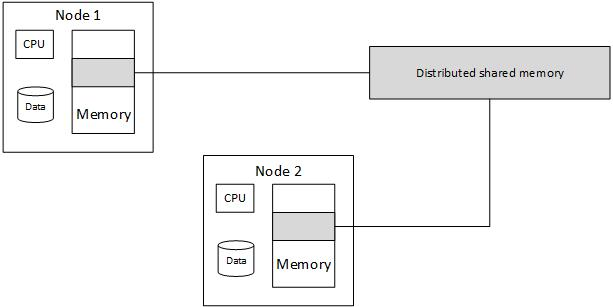
\includegraphics[width=0.8\textwidth,natwidth=610,natheight=642]{DistributedSharedMemory.jpg} 
	\captionsetup{format=plain,font=footnotesize,labelfont={bf,defaultCapFont},labelsep=quad,singlelinecheck=no}
	\caption[Distributed Computing System with 2 nodes]{
		\label{fig:distributedSharedMemory} 
		\footnotesize{%
			A distributed shared memory system with 2 nodes.
		}
	}
\end{figure}

The primary advantage of DSM is the shared memory abstraction provided. This gives the illusion of physically shared memory and allows developers to use the shared-memory paradigm, without having to think about communication mechanisms. For this reason the DSM paradigm is fully decoupled in space, since producers and consumers of data remain anonymous to each other, and in time, since the producers needs no knowledge of future use of the data. Synchronization decoupling is achieved by some implementations of DSM, where each node keeps local copies of the shared data~\cite{guedes1993distributed}.

A downside to the DSM abstraction is that it introduces overhead to the system, since the DSM abstraction has limited knowledge of the application flow, compared to communication via message passing~\cite{lu1995message}. 

 

%DSM pass by reference

%In distribted system there might be scenarios in which a task waits for a service at the queue of one resource, while at the same time another resource which is capable of serving the task is idle. The purpose of a load balancing algorithm is to prevent these scenarios as much as possible.

%three phases.
%Information collection: Gathers info of workload
%decision making: Calc optimal data dist.
%data migration: Transfer excess amount of workload from on overloaded processor to another underloaded processor

%Centralized: Size of grid increases, keppeing all the inforation about the state of all the resources is a bottlebeck. Scalability becomes an issue. Page 281. 

%The benifits of this technique stems from Load Balancing
%State Broadcast Algorithm (SBA). Page 282

%Basic assumptions Page 289.

%Scalability and makespan (Y). Page 298, conclusion.


\subsection{Publish/subscribe}

Publish/subscribe is a messaging pattern where communication is interest based instead of address based. Messages are characterized into classes and sent by publishers, without knowledge of how many subscribers there may be. Nodes can then subscribe to one or more classes of interest, without knowledge of how many publishers there are, providing a more decoupled, scalable and flexible interaction model.

\begin{figure}
	\centering
	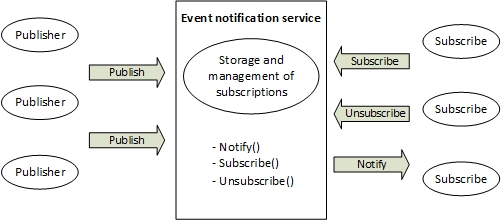
\includegraphics[width=0.9\textwidth,natwidth=610,natheight=642]{PublishSubscribe.jpg} 
	\captionsetup{format=plain,font=footnotesize,labelfont={bf,defaultCapFont},labelsep=quad,singlelinecheck=no}
	\caption[Distributed Computing System with 2 nodes]{
		\label{fig:publishSubscribe} 
		\footnotesize{%
			A simple publish/subscribe system.
		}
	}
\end{figure}

The publish/subscribe paradigm is event driven and corresponds to the observer design pattern, where subscribers are registered via keywords instead of registering their interest directly with the publishers. The paradigm relies on an event notification service providing storage and management for subscriptions and efficient delivery of events, as illustrated in \cref{fig:publishSubscribe}. The subscribers are notified subsequently of any event, generated by a publisher, matching the registered interest. The strength of this event-based communication is the full decoupling in time, space and synchronization between publishers and subscribers~\cite{eugster2003many}.

%Quality of service??

% DSM is only space and time decoupled but not sync, because consumers pull from shared space in a synchronous style


\subsection{Remote procedure call}
\label{sec:analysis:rpc}
Remote procedure call (RPC) is a communications paradigm built for client/server architecture~\cite{Microsoft2003RPC}, which makes remote interactions appear the same way as local interactions. The goal is to make the process of executing code on a remote machine as simple as calling a local function~\cite{dusseau2014intro} by factoring out common tasks, such as security, synchronization, and data flow handling. This explains the paradigms popularity in distributed systems. However distribution cannot be made completely transparent to the application, because it gives rise to further types of potential failures, like communication failures, that have to be dealt with explicitly~\cite{coulouris2005distributed}. 

The idea of RPC is quite simple. When a remote procedure is invoked, the calling environment is suspended, the parameters are passed across the network to the environment where the procedure is to execute and the desired procedure is executed at that location. When execution is finished, return values are sent back to the calling environment, where execution resumes~\cite{birrell1984implementing}.

A shortcoming of RPC is the strong coupling in time, space and synchronization. Although solutions have been presented to remove the synchronization coupling by future remote invocation. Remote method invocation is a paradigm where RPC as been applied to object-oriented contexts~\cite{eugster2003many}.

%Not appropriate for broadcasting

%Strong time coupled 
%sync coupled from the consumer side (waits for the return of the call, calling environment is suspended). Can be changed so sender does not expect reply (weak reliablity, no success or failure). Or return handle for sender to later request return value when needed (future remote invocation)

%Space coupling (remote reference to object)


%\section{Notification}
%
%The notification paradigm corresponds to the observer design pattern. It works by having subscribers register their interest directly with the publishers, which manages subscriptions and send events. It is usually implemented using two asynchronous invocations, in order to enforce synchronization decoupling: the first is sent by the client to the server, containing invocation arguments and a callback reference to the client, and the second is sent by the server to the client to return one or more replies. However publishers and subscribers remain coupled in time and space. Furthermore the communication management is left to the publisher. This can become a problem as the system grows in size~\cite{eugster2003many}.

%Publish/Subscribe where subscribers register their interest directly with publishers, which manages subscriptions and send events.

%event driven

%\section{Message queuing}
%Message queuing is a message-centric approach that usually integrate some form of publish/subscribe transaction. It works by having producers append messages to a global FIFO or priority queue asynchronously and consumers dequeue them synchronously from that same queue, where messages can only be consumed by one consumer. At an interaction level message queues recall much of DSM, where producers feed messages to some global memory space. Similarly to DSM, producers and consumers are decoupled in both space and time, where synchronous decoupling is only present for the producers~\cite{eugster2003many}.

%Global FIFO kø. Til hvis man er ligeglad med, hvem der tager opgaven??


%\begin{table}
%	\begin{tabular}{l >{\centering}m{5cm} c}
%		\hline
%		\hline
%		\textbf{Abstraction} & \textbf{Space} & \textbf{Time} & \textbf{Flow} \\
%		\hline
%		\hline
%		Message Passing & \checkmark & \checkmark \\
%		\hline
%		RPC/RMI & \checkmark & \checkmark \\
%		\hlines
%		Async. RPC/RMI & \checkmark & \checkmark \\
%		\hline
%		Future RPC/RMI & \checkmark & \checkmark \\
%		\hline
%		Notifications & \text{x}& \text{x} & \checkmark \\
%		\hline
%		DSM & \checkmark & \checkmark & P(\checkmark) \\
%		\hline
%		Message Queuing (PULL) & \checkmark & \checkmark & \text{P(} \checkmark \text{)} \\
%		\hline
%		Public/Subscribe & \checkmark & \checkmark & \checkmark \\
%		\hline
%		\hline
%	\end{tabular}
%	
%	\caption[MongoDB VoltDB]{
%		\label{tab:mongovolt}
%		\footnotesize{%
%			Comparison of MongoDB and VoltDB.
%		} 
%	}
%\end{table}

\subsection{Comparison with regards to the Siemens case}\label{distCompSiemensCaseComparison}

Looking at the Siemens case (\cref{sec:SiemensCase}) the new distributed system must act as a single unit, be able to perform park regulations and scale easily with the number of turbines. Furthermore Siemens wish to remove single point of failures. With this in mind, the remote procedure call paradigm is not an option because it is tight coupled and build for a client/server architecture, which is exactly what Siemens is trying to avoid. One could imaging using a partial client/server architecture, with a communication hierarchy, however this would introduce some communication overhead~\cite{Yu1997JavaDSM} and single point of failures to the system.

As mentioned, to perform the park regulation sequence, the wind farm needs a global shared state, where information about every turbine available to every turbine performing park regulations. Therefore, if the decentralized version of the Siemens case were to be implemented using raw message passing, it would result in building some kind of DSM and/or publish/subscribe abstraction, with roughly the same communication overhead. To save the trouble of developing this abstraction, we conclude that message passing is not an option as communication paradigm.

This leaves DSM and publish/subscribe as remaining paradigms. We present the following desired functionality of the chosen paradigm:
\begin{enumerate}
	\item Data must be copied and thus become locally available to all nodes in the system. This is to ensure that the regulation algorithm can be initiated without requesting data first. 
	\item Functionality 1. also means that data must be published to other nodes, such that a newly calculated state of a given turbine will automatically become available to every other turbine. 
	\item No locking of data when performing update operations. This is to ensure the regulation cycle can continue without being blocked by a turbine updating its state.
\end{enumerate}

One could imagine the Siemens case being implemented using either DSM or publish-subscribe. The abstraction of shared memory provided by DSM is attractive when looking looking at the Siemens case. As a system developer, being able to think of the global shared state as local memory is to prefer over event handling. However, publish behavior set by functionality 2. sounds like a publish-subscribe implementation. Therefore further investigation is needed in order to determine which one is preferred for the decentralized solution.

%The abstraction of shared memory provided by DSM is attractive when looking at the Siemens case. As a system developer, being able to think of the global shared state as local memory is to prefer over event handling. The Data Distribution Service defined by the Object Management Group provides a middleware based on Real Time Publish-Subscribe with the ability to maintain a history of messages. This enables the use of publish/subscribe as well as the ability to maintain a global shared state through the message history.

%This leaves DSM and publish/subscribe as remaining paradigms, where one could imagine the Siemens case being implemented using either of the two. The abstraction of shared memory provided by DSM is attractive when looking looking at the Siemens case. As a system developer, being able to think of the global shared state as local memory is to prefer over event handling. Therefore DSM is chosen over publish/subscribe since publish/subscribe introduces event handling to the system.

% The abstraction provided by DSM is attractive when looking looking at the Siemens case. As a system developer, being able to think of the global shared state as local memory is to prefer over thinking about communication semantics. However before before choosing, it is relevant to look at the cost of the DSM abstraction.

%\subsection{Message passing or DSM?}
%
%The abstraction provided by DSM is attractive when looking looking at the Siemens case. As a system developer, being able to think of the global shared state as local memory is to prefer over thinking about communication semantics. However before before choosing, it is relevant to look at the cost of the DSM abstraction.

%Comparing DSM with message passing in terms of processing time and network communication time is not entirely fair since DSM is an abstraction built using message passing. Therefore, Honghui~\cite{lu1995message} argues that it is hard for DSM to outperform message passing, in terms of application execution time, given the larger software-overhead. Honghui has studied and compared a DSM system with message passing system, with the goal to assess the differences in application development time and program execution time between DSM and message passing, and determine the causes of the lower program execution time of DSM systems. He ported 12 different parallel program scenarios to a DSM system called TreadMarks and a message passing system called PVM. For 5 of the scenarios, TreadMarks performed within 10\% of PVM. For 6 of the programs the difference were between 10\% - 30\%. For the last scenario, PVM performed twice as well as TreadMarks. 
%
%%He ported 12 different parallel program scenarios to a DSM system called TreadMarks and a message passing system called PVM and compared the two technologies with regards to programmability and performance. He argues that given DSM is an abstraction built on top of message passing, DSM cannot achieve better performance than message passing, given the larger software-overhead. Therefore the goal is to achieve the same performance as message passing using DSM. For 5 of the scenarios, TreadMarks performed within 10\% of PVM. For 6 of the programs the difference were between 10\% - 30\%. For the last scenario, PVM performed twice as well as TreadMarks. 
%
%Honghui argues that the program execution time is dependent of the logical flow of the program scenario. More messages and more data are sent in TreadMarks, explaining the performance differences. He gives the following reasons for the extra communication in TreadMarks:
%
%\begin{itemize}
%	\item Separation of synchronization and data transfer in TreadMarks. 
%	\item Extra messages to request updates for data in the invalidate protocol used in TreadMarks.
%	\item False sharing.
%	\item Diff accumulation for migratory data in TreadMarks.
%\end{itemize} 
%
%%1) Seperation of synchronization
%% Lazy release consistency: Against data races (which may result uin wrong results). Only the next processor that acquires the lock can access x --> only that processor is informormed of the change to x --> reduce message traffic. Ex: Barriers - No processor overites values before all processors have read the value computed in the previous interation.
%
%%2) Extra messages to request updates for data in the invalidate protocol used in TreadMarks
%% Memory page change communicatin. Modified pages are inviladated after an acquire. Later access causes access miss, which in turn causes installation of an up-to-date copy of the page.
%
%%3) False sharing
%% To objects er allokerede i samme memory page og de skrives til samtidig --> force update af page --> overhead
%
%%4) diff accumulation for migratory data in TreadMarks
%% Multiple-writer protocol to allow wrinting on same page at the same time. Uses a diff algorithm to reduce false sharing effects.
%
%Honghui concludes that the performance of a well optimized DSM system is comparable to that of a message passing system. Furthermore, development of systems with complex communication patterns takes a lot less effort using the DSM paradigm.
%
%In contrast to Honghui, Stumm and Zhou~\cite{stumm1990algorithms} argues that applications using DSM can in fact outperform their message passing counterparts, in a few cases. They argue, that this is possible for the following reasons:
%
%\begin{itemize}
% 	\item DSM algorithms typically move data on demand as they are being accessed, which spreads communication load over a longer period of time, allowing for a greater degree of concurrency. If for example a node uses the shared memory more than others, the node does not need to communicate for every write operation made to the shared memory.
% 	\item For DSM algorithms that sends data in large blocks, communication overhead is reduced. 
%\end{itemize} 
%
%Looking at the Siemens case the two major factors for the communication paradigm choice are scalability and availability.
%
%Message queuing and RMI offers feature which  



\subsection{State of the art DSM}

%With DSM chosen as the communication paradigm, this chapter describes, evaluates and discusses different DSM technologies in order to find the technology best suited for Siemens.
Looking for DSM frameworks for application level development, we are presented with with many types of In-Memory Databases (Redis~\cite{redis}, VoltDB~\cite{voltdb}, Gigaspaces XAP~\cite{gigaspacesxap}, ScaleOut Software~\cite{scaleout}, Hazelcast~\cite{hazelcast}, Oracle Coherence~\cite{oraclecoherence}, Memcached~\cite{memcached}, VMware Gemfire~\cite{gemfire}). In-Memory Databases (also known as Main Memory databases (MMDB)) are databases that stores data in memory. In a conventional database, disk data is primarily stored on the disk and may be cached into memory for access, where in a in-memory database, data is primarily stored in memory and may have a backup copy on the disk~\cite{garcia1992main}. MMDBs has a big potential for significant performance improvement over conventional databases, since there is virtually no I/O overhead for reading and writing the database, resulting in faster response time and improved throughput~\cite{lee2001single}.

All the above mentioned In-Memory Databases supports DSM behavior by copying stored data to all nodes of the system, thus making In-Memory Databases a potential for the decentralized solution. However, looking at functionality 1-3 mentioned in \cref{distCompSiemensCaseComparison}, using a database for handling communication is not will suited for the decentralized solution for the following reasons:

\begin{itemize}
	\item Most of the mentioned In-Memory Databases (Gigaspaces XAP~\cite{gigaspacesxap}, ScaleOut Software~\cite{scaleout}, Hazelcast~\cite{hazelcast}, Oracle Coherence~\cite{oraclecoherence}, Memcached~\cite{memcached}, VMware Gemfire~\cite{gemfire}) uses shared nothing (SN) architecture (also known as Sharding). SN is a distributed computing architecture where none of the nodes share memory or disk storage~\cite{stonebraker1986case}, thus without a single point of contention. For a In-Memeory Database this means that the database is partitioned throughout the nodes either by assigning different computers to deal with different users or queries, or by requiring every node to maintain its own copy of the application's data, using some kind of coordination protocol. This provides impressive scalability for a system using pure SN. However, since local copies of every state in the system is exactly what is desired for the decentralized solution, the SN architecture contradicts functionality 1. Furthermore, SN built databases introduces client-server architecture for broker implementation.
	\item Others (Redis~\cite{redis}, VoltDB~\cite{voltdb}, Memcached~\cite{memcached}) uses a client-server architecture, where a broker is needed to keep track of where data is located. This introduces single point of failures and broker communication, which brings a communication overhead to the system. 
	\item Database replication is not well suited for functionality 2. Database replication is built to ensure consistency between nodes, thus bringing an unnecessary overhead to the decentralized solution that results in increasing the regulation cycle time or, if lazy replication is used, late arrival of new states~\cite{wiesmann2000database}.
\end{itemize}

Another DSM framework found is TreadMarks~\cite{keleher1994treadmarks} created at Rice University in 1994. However, this software is outdated (the TreadMarks homepage gives a 404 Not Found).

Thus we conclude that frameworks implementing the DSM paradigm at application level is In-Memory Databases and not suited for the decentralized solution.

%Distributed memory. Only shared for replica reasons.
%Share nothing architecture

%casusally consistent: Writes that are potentially causally related must be seen by all processes in the same order. Concurrent writes may be seen in a different order on different machines.

%\subsubsection{AppFabric}
%Runs on IIS




%Standalone, avoid overhead


%\subsection{In memory databases}
%Client/server architecture

%\subsection{In-memory data grids}
%Distributed memory. Only shared for replica reasons


%\subsubsection{Oracle Coherence}
%dist. memory --> distributed chache
%java, .net, c++
%http://www.oracle.com/technetwork/middleware/coherence/distributed-caching-100021.html


%\subsubsection{VMware Gemfire}
%Contact sales
%Not open source

%\subsubsection{Gigaspaces XAP}
%Share nothing architecture

%\subsubsection{ScaleOut Software}
%Java, .NET, C/C++ 
%cash
%Share nothing architecture
%http://www.scaleoutsoftware.com/downloads-resources/downloads/

%\subsubsection{NCache}
%expensive
%http://www.alachisoft.com/ncache/index.html

%\subsubsection{Hazelcast}
%java
%opensource
%http://hazelcast.com/products/hazelcast/

%\subsubsection{Infinispan}
%promising

%\subsubsection{DSM in .NET}
%IP multicast

%casusally consistent: Writes that are potentially causally related must be seen by all processes in the same order. Concurrent writes may be seen in a different order on different machines.

%\subsubsection{AppFabric}
%Runs on IIS

\subsection{State of the art publish/subscribe}
\label{sec:stateArtPublish}
The following section contains a presentation of a number of publish/subscribe standards. Each standard will be evaluated and a one will be chosen as the best suited publish/subscribe standard for the decentralized solution.

\paragraph{Java Message Service} (JMS)~\cite{hapner2002java} is a messaging API that allows application components based on Java EE to exchange messages using either point-to-point communication or publish-subscribe. As JMS is an API specification the underlying message service responsible for the actual message handling can be any messaging service, as long as it implements the JMS Provider interface.

\begin{figure}[!h]
	\centering
	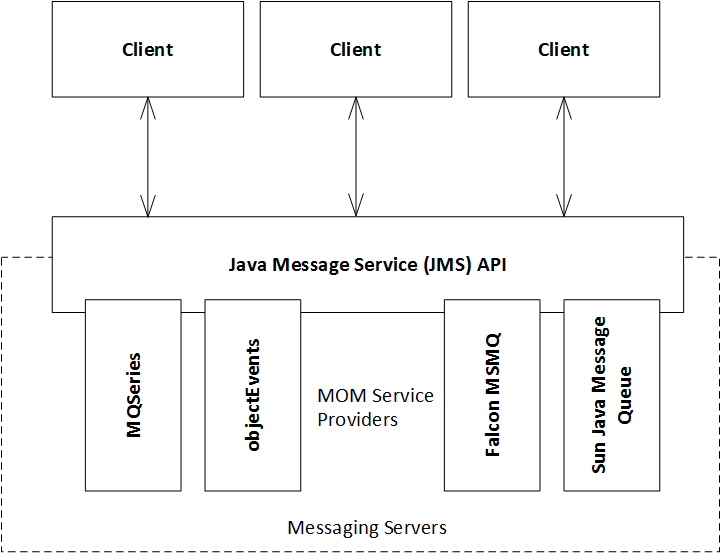
\includegraphics[width=0.6\textwidth,natwidth=610,natheight=642]{jmsArchitecture.png} 
	\captionsetup{format=plain,font=footnotesize,labelfont={bf,defaultCapFont},labelsep=quad,singlelinecheck=no}
	\caption[JMS overview]{
		\label{fig:jmsOverview} 
		\footnotesize{%
			JMS overview.
		}
	}
\end{figure}

JMS introduces a messaging server to facilitate communication between clients. This can be compared to the Park Pilots of the current Siemens system as the scalability of JMS will depend on how well the messaging server handles multiple clients. To avoid single points of failure multiple servers are needed for failover. Removing Park Pilots be decentralizing them and then adding JMS messaging servers to support publish/subscribe messaging may improve scalability but in the end we retain the centralized architecture where communication must flow through central points in the network which is not desirable. 

\paragraph{Common Object Request Broker Architecture Notification Service} (CORBA NS)~\cite{corbanotificationservicespecification} is an Object Management Group standard defining a publish subscribe service for the Common Object Request Broker Architecture (CORBA).
CORBA builds on the RPC paradigm described in~\cref{sec:analysis:rpc}.
CORBA addresses the problem of the strong coupling between components in RPC by introducing a Object Request Broker (ORB) as an intermediate between components and thereby decouple them from each other in space and synchronization terms. CORBA NS further decouples the components by removing the time coupling.

\begin{figure}[!h]
	\centering
	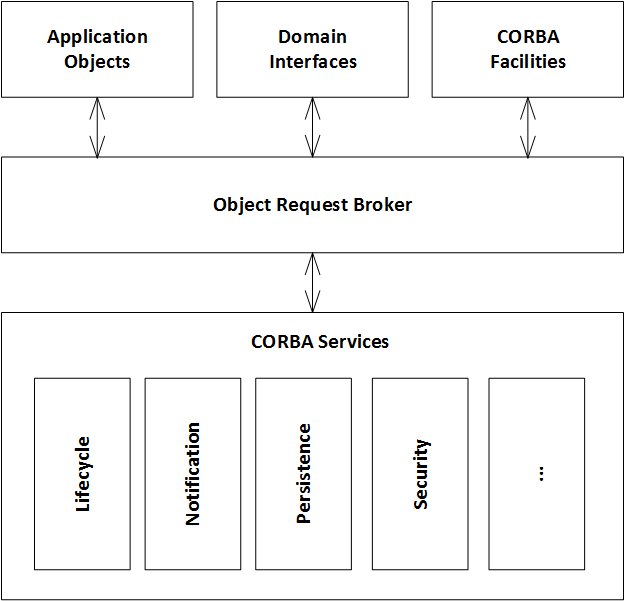
\includegraphics[width=0.6\textwidth,natwidth=610,natheight=642]{corbaArchitecture.png} 
	\captionsetup{format=plain,font=footnotesize,labelfont={bf,defaultCapFont},labelsep=quad,singlelinecheck=no}
	\caption[JMS overview]{
		\label{fig:corbaOverview} 
		\footnotesize{%
			CORBA overview.
		}
	}
\end{figure}

Thus, even though CORBA builds on the strong coupled paradigm of RPC full decoupling is possible when adding the ORB and CORBA NS abstractions. The many layers if abstractions is a problem when looking at the time of message propagation.
All messages must go through each abstraction layer at both the publisher and the subscriber side adding overhead to the message propagation time. Another problem with CORBA is the complexity of implementing it's API. As stated in ~\cite{Henning:2006:RFC:1142031.1142044}

"\textit{...CORBA's object adapter requires more than 200 lines of interface definitions, even though the same functionality can be provided in about 30 lines-the other 170 lines contribute nothing to functionality, but severely complicate program interactions with the CORBA runtime...}".

CORBA and CORBA NS has multiple features that are interesting for a decentralized version of the current Siemens system, unfortunately the complexity and added overhead makes CORBA NS less attractive.

\paragraph{Advanced Message Queuing Protocol}(AMQP)~\cite{amqp} is an open standard protocol for message-oriented middleware defined by the Organization for the Advancement of Structured Information Standards (OASIS). 
The standard defines an interoperability wire-protocol designed to support a wide variety of messaging applications. In order to use AMQP on the application level a client implementation of the AMQP protocol must be used. 
There are a number of client implementations in different languages~\cite{amqpimplementations}. AMQP sends messages via multiple message queues.

\begin{figure}[!h]
	\centering
	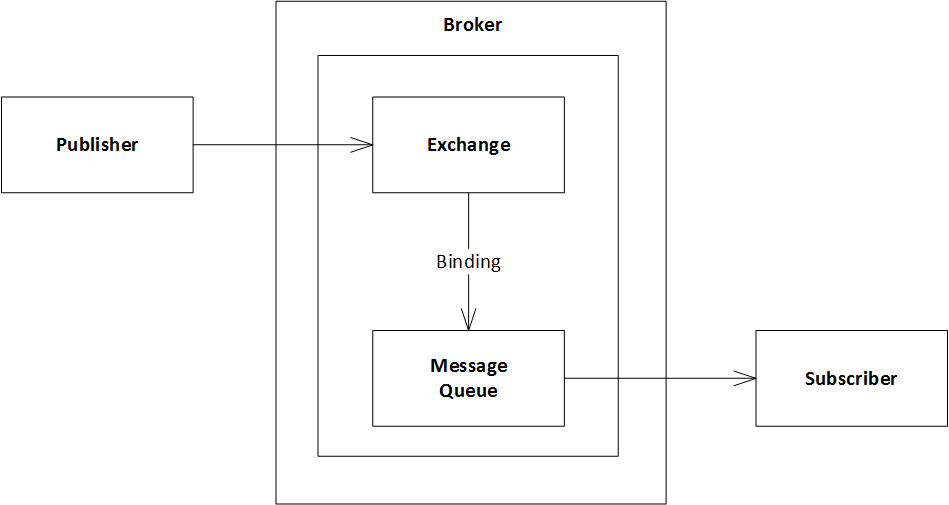
\includegraphics[width=0.6\textwidth,natwidth=610,natheight=642]{amqpArchitecture.png} 
	\captionsetup{format=plain,font=footnotesize,labelfont={bf,defaultCapFont},labelsep=quad,singlelinecheck=no}
	\caption[JMS overview]{
		\label{fig:amqpOverview} 
		\footnotesize{%
			AMQP overview.
		}
	}
\end{figure}

A message has a routing key that decides which queue it is to enter in order to reach the subscribers of the message. Using a broker in a decentralized architecture may cause problems if the number of messages that is sent in the network exceed the capacity of the broker.
The broker is a single point of failure which is unfortunate since this thesis aims to remove single point of failures from the current Siemens system.

\paragraph{Data Distribution Service for Real-Time Systems} (DDS) is an Object Management Group standard defining a middleware for communication between information provideres and information consumers.
The standard is an API specification and an interoperability wire-protocol that defines a data-centric publish-subscribe architecture~\cite{pardo2003omg}.

\begin{figure}[!h]
	\centering
	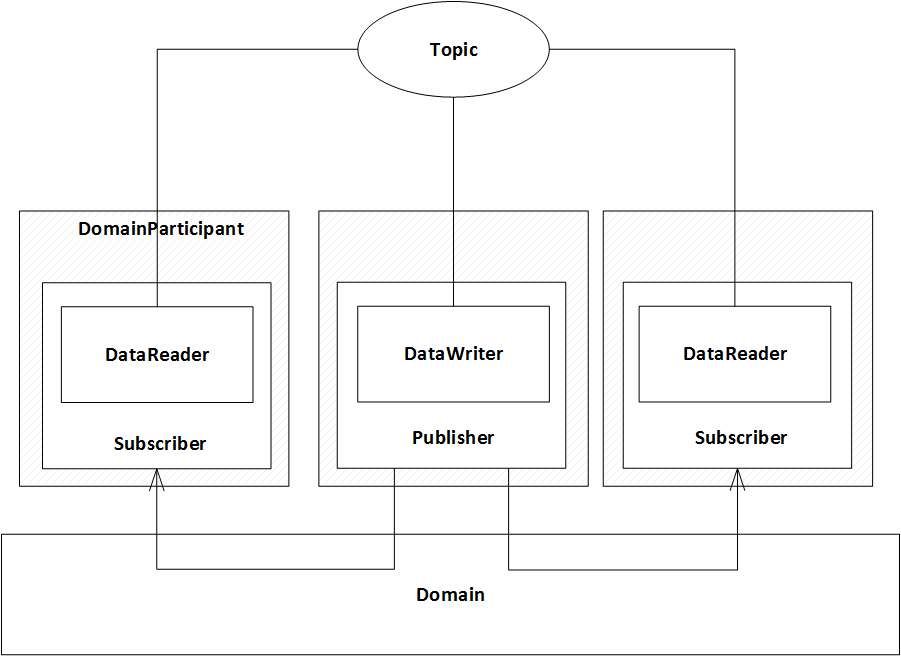
\includegraphics[width=0.6\textwidth,natwidth=610,natheight=642]{ddsArchitecture.png} 
	\captionsetup{format=plain,font=footnotesize,labelfont={bf,defaultCapFont},labelsep=quad,singlelinecheck=no}
	\caption[JMS overview]{
		\label{fig:ddsOverview} 
		\footnotesize{%
			DDS overview.
		}
	}
\end{figure}

DDS has no central broker meaning all cache and queuing of messages happens at the client. As there is no central broker clients sends messages directly to each other using multicast in order to limit the number of packages in the network. The decentral architecture of DDS allows for great scalability since there is no central points that will be congested if the number of packages in the network increase.

As DDS is the best candidate for a middleware for the decentralized solution it will be presented in depth in the following section.
%As DDS is the best candidate for a middleware for the decentralized solution it will be investigated in depth in the following section to ensure it's ability to scale.

\section{Data Distribution Service for Real-Time Systems}
\label{sec:DDS}
The DDS standard provides a number of services that a decentralized system like the one this thesis aims to create could profit from.
Services include amongst others:

\begin{itemize}
	\item Automatic node discovery
	\item A data-centric publish-subscribe approach that allows for distribution of data by topics, decoupling the nodes of the system
	\item Cross-platform support
	\item Fine grained control of Quality of Service parameters
\end{itemize}

DDS relies on the multicast features of the IP protocol which is described below.

\subsection{IP Protocol Addressing Methodologies}

\begin{wrapfigure}{r}{0.225\textwidth}
	\vspace{-20pt}
		\tikzstyle{fact}=[rectangle, draw=none, rounded corners=1mm, fill=blue, drop shadow,
	text centered, anchor=north, text=white]
	\tikzstyle{source}=[circle, draw=none, fill=orange, circular drop shadow,
	text centered, anchor=north, text=white]
	\tikzstyle{target}=[circle, draw=none, fill=blue, circular drop shadow,
	text centered, anchor=north, text=white]
	\tikzstyle{other}=[circle, draw=black!50, fill=white, circular drop shadow,
	text centered, anchor=north, text=white]
	%\tikzstyle{comment}=[rectangle, draw=black, fill=black!60, rounded corners, drop shadow,
	%anchor=west, text=white, text width=6.5cm]
	\begin{tikzpicture}[node distance=0.8cm]
		\node (Source) [source] {};
		\node (Target1) [target,right=of Source] {} edge [<-] (Source);
		\node (Target2) [other,above=of Target1] {};
		\node (Target3) [other,below=of Target1] {};
		\node (Target3) [other,above=of Source] {};
		\node (Target3) [other,below=of Source] {};
		
		\begin{pgfonlayer}{background}
			\path (Source.west |- Target2.north)+(-0.4,0.4) node (a) {};
			\path (Target1.east |- Target3.south)+(0.4,-0.4) node (b) {};
			\path [fill=yellow!40,rounded corners, draw=black!50, dashed] (a) rectangle (b); 
		\end{pgfonlayer}
	\end{tikzpicture}
	\caption{Unitcast}
	\label{fig:networkUnicast}
	
	\vspace{10pt}
		\begin{tikzpicture}[node distance=0.8cm]	
		\node (Source) [source] {};
		\node (Target1) [target,right=of Source] {} edge [<-] (Source);
		\node (Target2) [target,above=of Target1] {} edge [<-] (Source);
		\node (Target3) [target,below=of Target1] {} edge [<-] (Source);
		\node (Target3) [target,above=of Source] {} edge [<-] (Source);
		\node (Target3) [target,below=of Source] {} edge [<-] (Source);
		
		\begin{pgfonlayer}{background}
			\path (Source.west |- Target2.north)+(-0.4,0.4) node (a) {};
			\path (Target1.east |- Target3.south)+(0.4,-0.4) node (b) {};
			\path [fill=yellow!40,rounded corners, draw=black!50, dashed] (a) rectangle (b); 
		\end{pgfonlayer}
	\end{tikzpicture}
	\caption{Broadcast}
	\label{fig:networkBroadcast}
			
	\vspace{10pt}
	\begin{tikzpicture}[node distance=0.8cm]	
		\node (Source) [source] {};
		\node (Target1) [target,right=of Source] {} edge [<-] (Source);
		\node (Target2) [target,above=of Target1] {} edge [<-] (Source);
		\node (Target3) [other,below=of Target1] {};
		\node (Target3) [other,above=of Source] {};
		\node (Target3) [target,below=of Source] {} edge [<-] (Source);
		
		\begin{pgfonlayer}{background}
			\path (Source.west |- Target2.north)+(-0.4,0.4) node (a) {};
			\path (Target1.east |- Target3.south)+(0.4,-0.4) node (b) {};
			\path [fill=yellow!40,rounded corners, draw=black!50, dashed] (a) rectangle (b); 
		\end{pgfonlayer}
	\end{tikzpicture}
	\caption{Multicast}
	\label{fig:networkMulticast}
		
	\vspace{-10pt}
\end{wrapfigure}

The IP protocol defines different communication methodologies among these are: Unicast, Broadcast~\cite{RFC0919_Broadcast} and Multicast~\cite{RFC1112_Multicast_IGMPv1}.
These methodologies each allow for different kinds of communication.

\paragraph{Unicast} is the simplest and most used methodology, it is provides point to point communication and is the basis for most TCP/IP communication.
% most TCP/IP since it is also used in Anycast
As seen in \cref{fig:networkUnicast} the source node only send packet to one node, this kind of communication works well as long as the data being transfered only needs to be sent to one node.
%\paragraph{Anycast} exsists but is irelevant to our project

\paragraph{Broadcast} is the direct opposite of unicast, it provides one to all communication, illustrated in \cref{fig:networkBroadcast}. All in this context mens all machines on the same subnet or locally behind the nearest router.
The source node only needs to send one packet to reach every other node, copying of the packet is done in the network by switches and routers.
There exist a broadcast address for every subnet and a special address which broadcast to all machines within the local network separated from the outside with a router.
%The broadcast address for a given subnet can be found by doing a bitwise or operation on the local ip address with the binary complement of the subnet mask ($broadcast~address~=~local~ip~|~!subnet~mask$). To broadcast to all subnets behind the nearest router the address $255.255.255$ can be used, other protocols have similar capabilities.
Broadcast does not support TCP/IP and delivers packet in a best effort way, this means that there is no guarantee or feedback of if the packet arrived, all this has to be built on top if needed.
On large networks there can be a lot of broadcast traffic that every node needs to decide if it needs to respond to or discard.
In the new IPv6 broadcast is no longer supported~\cite{RFC4291_AddressingIPv6Draft} and is replaced by multicast protocols, this makes it optional to listen to broadcast traffic and possibly increase performance.

\paragraph{Multicast} is a combination of unicast and broadcast and can be configured to be used as either one, however this is not what it is designed for. Multicast is designed to provide one to many communication as illustrated in \cref{fig:networkMulticast}.
Multicasting works using multicast groups, these groups are maintained by routers and layer 2 switches. The way a node is added to a multicast group is by transmitting a packet requesting a group membership using the IGMP protocol. Each multicast group is associated with a multicast ip address, this ip address is used by the transmitting node when a packet is to be transmitted to a multicast group.
Communicating via multicating is efficient and ensures that each node can be configured to handle a minimum number of packets, routers and switches however has a added responsibility of maintaining information of which multicast address each port is associated with and transmitting packets to all of them.

\subsection{Main DDS entities}
RTI Connext provides a number of entities that must be present in a system in order to enable commmunication.

\begin{itemize}
	\item \textbf{DomainParticipant} \\
		\textit{Domains} represent logical, isolated, communication networks. Entities existing in different \textit{Domains} are unable to communicate with each other. The \textit{DomainParticipant} is created with an integer value specifying the \textit{Domain} it belongs to. The \textit{DomainParticipants} owns the \textit{Topics}, \textit{Publishers} and \textit{Subscribers} in effect making them belong to a specific \textit{Domain}.
	
	\item \textbf{Publisher} \\
		A \textit{Publisher} owns and manages a number of \textit{DataWriters}. The \textit{Publisher} is responsible for the publishing of data provided by the \textit{DataWriters}. One \textit{Publisher} can publish data from several \textit{DataWriters} on several different \textit{Topics}.
	
	\item \textbf{Subscriber} \\
		A \textit{Subscriber} owns and manages a number of \textit{DataReaders}. The \textit{Subscriber} is responsible for the receipt of published data on behalf of the \textit{DataReaders}. One \textit{Subscriber} can receive data for several \textit{DataReaders} on several different \textit{Topics}. 
	
	\item \textbf{Topic} \\
		\textit{Topics} interconnect \textit{DataReaders} and \textit{DataWriters}. \textit{DataWriters} can subscribe to a \textit{Topic} and receive data each time a \textit{DataReader} publishes data to the same \textit{Topic}.
	
	\item \textbf{DataWriter} \\
		A \textit{Datawriter} is owned by a single \textit{Publisher}. It is associated with a single \textit{Topic} and is able to send data to this \textit{Topic} using the owning \textit{Publisher}.
	
	\item \textbf{DataReader} \\
		A \textit{DataReader} is owned by a single \textit{Subscriber}. It is associated with a single \textit{Topic} and is able to receive data published to this \textit{Topic} using the owning \textit{DataReader}.
\end{itemize}

\begin{figure}
	\centering
	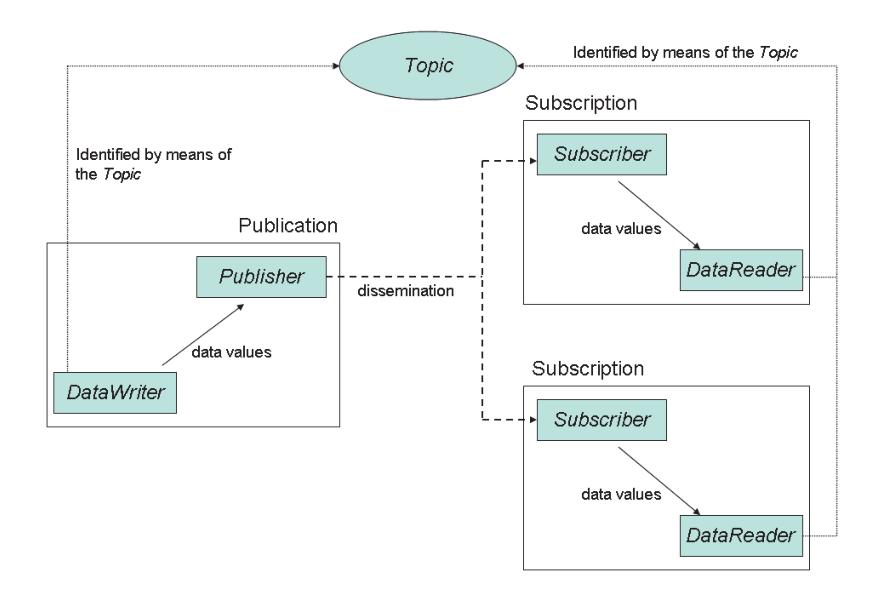
\includegraphics[width=0.7\textwidth,natwidth=610,natheight=642]{DDSentities.png} 
	\captionsetup{format=plain,font=footnotesize,labelfont={bf,defaultCapFont},labelsep=quad,singlelinecheck=no}
	\caption[DDS entities]{
		\label{fig:ddsEntities} 
		\footnotesize{%
			DDS entites as presented in RTI Connext Core Libraries and Utilities User's Manual~\cite{rtiConnextUsersManual}.
		}
	}
\end{figure}

\subsection{Node discovery}
Node discovery in DDS is performed using the Simple Discovery Protocol(SDP).
This protocol describes a sequence of messages that are sent between DDS entities in order for them to automatically discover each other.
Node discovery is important in a system like the Siemens Case described in \cref{sec:SiemensCase} because the regulation of a wind farm requires data from all turbines in order to regulate the overall wind farm production correctly.
The protocol is split into two phases:

\begin{itemize}
	\item Simple Participant Discovery Protocol
	\item Simple Endpoint Discovery Protocol
\end{itemize}

The Simple Participant Discovery Protocol(SPDP) phase facilitates the discovery of \textit{DomainParticipants} across the network.
After this phase has been completed all \textit{DomainParticipants} in the system has registered the necessary information to enable future communication with each other.

The Simple Endpoint Discovery Protocol(SEDP) phase facilitates the discovery of \textit{DataWriters} and \textit{DataReaders} across the network.
After this phase has been completed all \textit{DomainParticipants} in the system has registered the necessesary information to enable \textit{DataWriters} and \textit{DataReaders} to communicate.

\begin{figure}
	\centering
	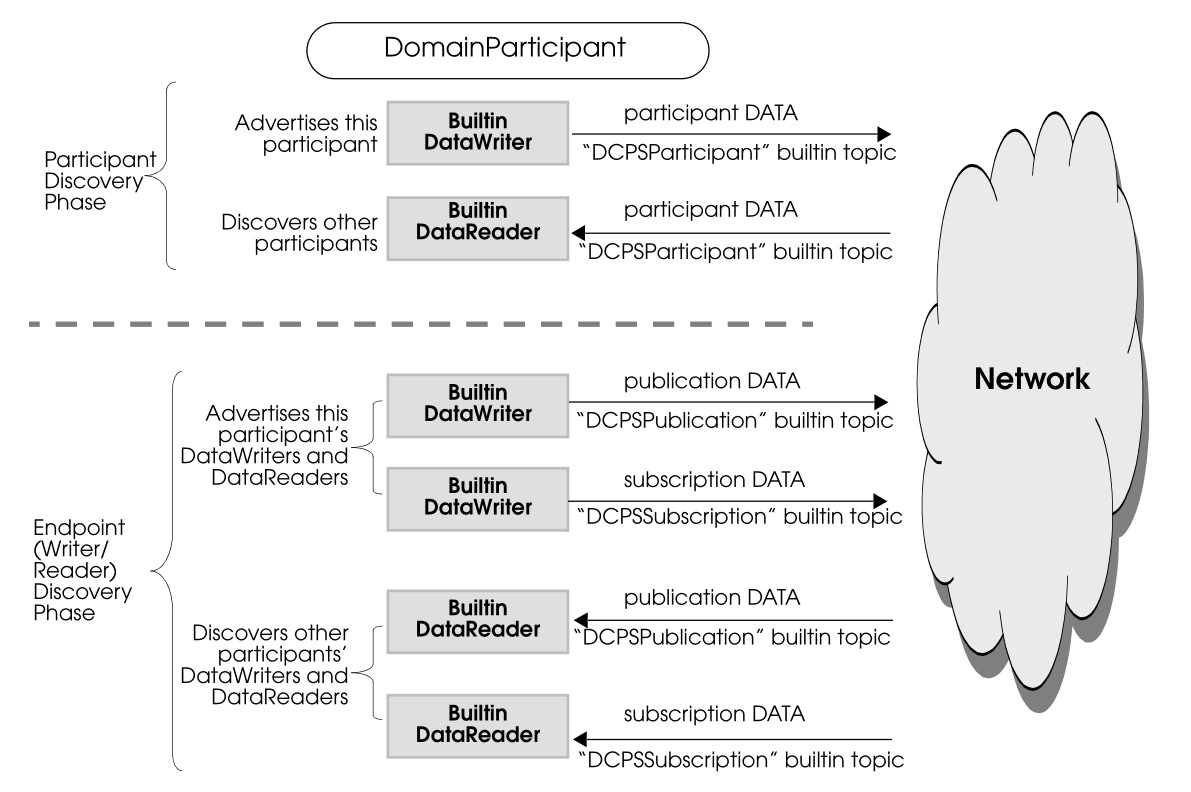
\includegraphics[width=0.7\textwidth,natwidth=610,natheight=642]{DDSdiscovery.png} 
	\captionsetup{format=plain,font=footnotesize,labelfont={bf,defaultCapFont},labelsep=quad,singlelinecheck=no}
	\caption[DDS discovery phases]{
		\label{fig:DDSdiscovery} 
		\footnotesize{%
			DDS discovery phases as presented in RTI Connext Core Libraries and Utilities User's Manual~\cite{rtiConnextUsersManual}.
		}
	}
\end{figure}

Since the SEDP registers all the \textit{DataWriters} and \textit{DataReaders} in the system the protocol scales poorly~\cite{(CFDP)}. The discovery time and number of packets sent grows as the number of endpoints increase. This affects the scalability of the system directly. To avoid the increase in discovery time different protocols has been proposed to solve the scalability problem. 

\paragraph{Content-based Filtering Discovery Protocol(CFDP)} is similar to SDP during the SPDP phase but it differs in the SEDP phase where changes has been made in order to facilitate content-based discovery of endpoints. The filtering allows the \textit{DomainParticipant} to reduce the number of discovery messages to the number of endpoints that needs to communicate with the \textit{DomainParticipant} and its local endpoints. Currently CFDP has only been tested using unicast and here the protocol outperforms SDP in terms of network usage, packages sent and discovery time. However if multicast is used as the underlying transport protocol SDP outperforms CFDP. This happens because SDP only needs one multicast for all \textit{DomainParticipants}. CFDP in contrast will need one multicast address for each content filter used. This limitation in CFDP is proposed as a subject for further research.

Since CFDP does not outperform SDP when using multicast, CFDP is not suited as the discovery protocol for the system described in this thesis.

\paragraph{A discovery protocol based on Bloom filters} has been proposed as well~\cite{monedero2009dds}. Similar to CFDP the Bloom filter approach aims to reduce the number of packets that needs to be exchanged in order to discover endpoints in the system. The Bloom filter approach introduces a Bloom filter for each \textit{DomainParticipant} that contains information describing the local endpoints. During the SPDP phase the Bloom filters are distributed to all \textit{DomainParticipants}. In this way information of all endpoints in the system has been distributed when the SEDP phase begins allowing the \textit{DomainParticipants} to decrease the number of discovery messages sent to the number of endpoints that it must know in order to facilitate communication for its local \textit{DataReaders} and \textit{DataWriters}. 

Again the main advantage of using Bloom filters is found in the unicast scenario. In a multicast scenario there still are advantages of using the Bloom filter approach because the \textit{DomainParticipants} are able to limit the number of discovery messages compared to SDP. The advantage of using the Bloom filter approach increases as the ratio between endpoints and \textit{DomainParticipants} increase.

Since a wind farm has a limited number of endpoints, less than 300 turbines, the decrease in discovery time by using the Bloom filter approach would be minor. Therefore the Bloom filter approach is not further investigated in this thesis. \newline

The Simple Discovery Protocol does not scale well with the number of endpoints. This problem is currently under research and solutions have been proposed. As of the time of writing none of the proposed solutions to the problem are well suited for use in this thesis. Further research in the area may present new solutions to the problem that are well suited for use in a multicast enabled system with less than 300 nodes.

\subsection{Quality of Service}
DDS provides Quality of Service(QoS) parameters to enable very fine grained control over the behavior of the deployed DDS entities in a system. To create a decentralized system several of the QoS parameters are interesting.

\begin{itemize}
	\item \textbf{Multicast} \\
		Enabling multicast in the system will decrease the network traffic in the system, which in turn increases scalability.
		
	\item \textbf{History} \\
		The History parameter will enable the system to keep a log of messages received during operation thus eliminating the need for another storage option. This saves the system from using additional resources for storing and retrieving values from a file or a local database.
		
	\item \textbf{Lifespan} \\
		The History parameter enables the system to keep a log of messages but the history may only be relevant for a specified amount of time. In order not to keep irrelevant messages it can be specified how long they are relevant.
	
	\item \textbf{Durability} \\
		To make sure a new turbine can start operation the Durability parameter can be used in order to update the new turbine with the history of messages in the system. In this way the turbine does not need to wait to receive new data from individual turbines to start regulation, instead it can start regulation as soon as the history is received.
		
	\item \textbf{Reliability} \\
		This parameter regulates the reliable delivery of messages in the system, which affect the operation of the turbines and their regulation.
		
	\item \textbf{Liveness} \\
		The Liveness parameter specifies how liveness of a \textit{DataWriter} is determined. This allows the system to detect when a turbine is no longer available and to respond in an appropriate way.
\end{itemize}

Using the QoS of DDS a system can be configured to fit its environment and its requirements very tightly allowing efficient and reliable operation. QoS will be elaborated further in chapters \cref{cha:existingSystem} and \cref{cha:decentralizedSystem}.

\subsection{Conclusion}
The Data Distribution Service enables both communication using publish/subscribe as well as the ability to maintain a global shared state by preserving message history. Coupled with the fact that the middleware provides automatic node discovery, cross-platform support and fine grained control using Quality of Service parameters the Data Distribution Service is the best choice of middleware for the Siemens Case (\cref{sec:SiemensCase}).
